%----------------------------------------------------------------------------------------
%	CONFIGURATIONS
%----------------------------------------------------------------------------------------

\documentclass[10pt,a4paper,oneside]{article}

\usepackage[utf8]{inputenc}
\usepackage{graphicx}
\usepackage{epstopdf}
\usepackage{natbib}
\usepackage{amsmath}
\usepackage{multirow}
\usepackage{lipsum}
\usepackage{caption}
\usepackage{subcaption}
\usepackage{float}
\usepackage[a4paper,left=2cm,right=2cm,top=2.5cm,bottom=2.5cm]{geometry}

%----------------------------------------------------------------------------------------
%	INFORMATION
%----------------------------------------------------------------------------------------

\title{Estudo de paralelismo num problema de simulação discreta}

\author{Filipe Figueiredo\footnote{Filipe Figueiredo - 201203559},
  Pedro Paredes\footnote{Pedro Paredes - 201205725}, DCC - FCUP}

\date{Dezembro 2015}

\renewcommand{\tablename}{Tabela}
\renewcommand{\figurename}{Figura}
\renewcommand{\refname}{Referências}
\newcommand{\BigO}[1]{\mathcal{O}(#1)}

\makeatletter
\makeatother

\begin{document}

\maketitle

%----------------------------------------------------------------------------------------
%	SECTION 1
%----------------------------------------------------------------------------------------

\section{Introdução}
\label{sec:intro}
Neste trabalho discutimos um problema de simulação de eventos
discretos determinística numa grelha e exploramos diferentes
estratégias de paralelismo possíveis.

Este tipo de problemas é notoriamente difícil de se paralelizar devido
às dependências existentes nos dados e na topologia da simulação
provenientes das restrições impostas pelo problema. Neste trabalho, a
topologia da simulação é regular (uma grelha retangular) o que permite
que abordagens simples sejam efetivas, mas no geral é necessário
recorrer a métodos mais complexos como computação especulativa.

Focamo-nos em três abordagem simples, que aproveitam diferentes
aspetos do problema. Além disso, exploramos diferentes esquemas de
redistribuição de trabalho de modo a podermos manter eficiência em
\textit{inputs} desbalanceados.

O resto deste relatório será organizado da seguinte forma. Na
Secção~\ref{sec:prob} descrevemos o problema com algum pormenor e as
dificuldades em o paralelizar. Na Secção~\ref{sec:par} introduzimos as
estratégias para paralelizar o problema e fazemos uma comparação
teórica entre elas. Na Secção~\ref{sec:res} apresentamos os resultados
experimentais obtidos pela implementação de cada estratégia referida
na secção anterior. Finalmente, na Secção~\ref{sec:con} fazemos
algumas notas finais.

%----------------------------------------------------------------------------------------
%	SECTION 2
%----------------------------------------------------------------------------------------

\section{Descrição do problema}
\label{sec:prob}
O problema que pretendemos estudar é uma simulação numa grelha
retangular de $R$ linhas por $C$ colunas. Cada célula da grelha pode
estar vazia ou conter um dos seguintes elementos: uma pedra, um coelho
ou uma raposa. A simulação é feita iterativamente, ou seja, a partir
de uma geração inicial (o \textit{input}), representada por uma
distribuição de pedras, coelhos e raposas numa grelha, é gerada uma
nova geração seguindo um conjunto de regras fechado e o mesmo é
repetido $N_G$ vezes até se obter a geração final (o
\textit{output}). Representamos por $N_i$ o número de coelhos e
raposas existentes na geração $i$.

As regras de construção de uma nova geração começam por primeiro mover
todos os coelhos simultaneamente para uma nova célula que esteja
vazia, seguindo uma ordem determinística. Seguidamente as raposas são
movidas para uma célula vazia ou para uma célula que contenha um
coelho. O último caso representa uma raposa a comer um coelho, o que
na prática significa que o coelho que foi comido desaparece da
simulação na nova geração. Adicionalmente, tanto os coelhos como as
raposas podem procriar, duplicando-se cada animal num período
regular. A Figura~\ref{fig:sim} exemplifica duas gerações de uma
simulação.

\begin{figure}[H]
    \centering
    \begin{subfigure}[b]{0.4\textwidth}
      \centering
      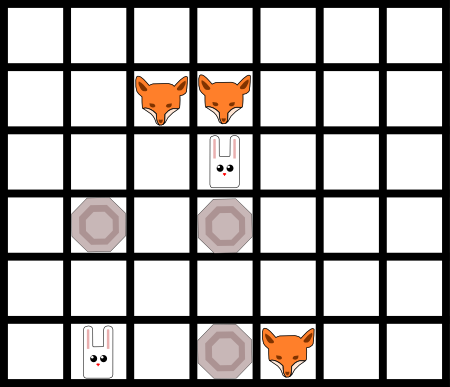
\includegraphics[height=1.6in]{grid1.png}
    \end{subfigure}
    ~
    \begin{subfigure}[b]{0.4\textwidth}
      \centering
      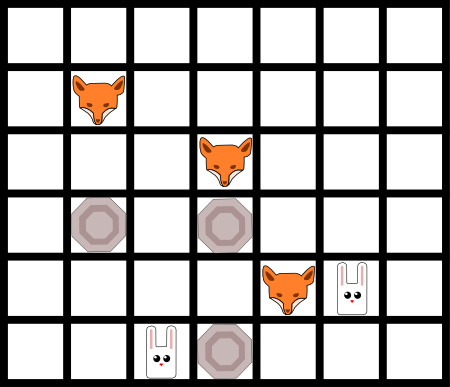
\includegraphics[height=1.6in]{grid2.png}
    \end{subfigure}
    \caption{Exemplo de duas gerações de uma simulação}
    \label{fig:sim}
\end{figure}

A partir desta descrição simples do problema é possível identificar
dependências fortes do problema. Em cada nova geração, a simulação das
raposas só pode ser iniciada após a conclusão da simulação de todos os
coelhos, pois os movimentos dos coelhos condicionam os movimentos das
raposas (a dependência é apenas local, ou seja, um coelho muito
afastado de uma certa raposa não condiciona o seu movimento, mas
aproveitar este tipo de observações requer um algoritmo mais complexo
e menos óbvio de paralelizar e não foi por isso considerado). Assim,
existe aqui um ponto de sincronização necessário na execução da
simulação.

Adicionalmente, a simulação dos coelhos também impõe certas restrições
nos movimentos dos coelhos entre si. Além de serem obstáculos uns para
os outros, podem existir conflitos no movimento de dois ou mais
coelhos que se podem movimentar para a mesma célula. Nesse caso apenas
um coelho sobrevive e por isso é necessário sincronizar os coelhos que
após a resolução de conflitos se mantêm. Isto é análogo para as
raposas.

É de notar que este tipo de simulação tem uma natureza exponencial
associada. Apesar de ser possível limitar o crescimento dos coelhos e
raposas atribuindo-lhes valores altos para o período para procriação,
as simulações mais ``interessantes'' (leia-se mais movimentadas)
rapidamente (em poucas gerações) preenchem a grelha a mais de
$50\%$. Por esta razão, não consideramos representações esparsas da
grelha (isto é, que não guardam a grelha diretamente como uma matriz),
pois além de serem menos eficientes têm aplicabilidade reduzida.

%----------------------------------------------------------------------------------------
%	SECTION 3
%----------------------------------------------------------------------------------------

\section{Estratégias de paralelização}
\label{sec:par}
Discutiremos três abordagens com diferentes focos e as suas vantagens
e desvantagens. A primeira abordagem (no código corresponde a
\texttt{TopologyEngine}) é uma abordagem orientada à topologia do
problema (ou \textit{topology driven parallelism}), ou seja, passa por
paralelizar o problema usando a grelha que serve de base da
simulação. A segunda estratégia (no código corresponde a
\texttt{DDEngine}) é orientada aos dados do problema (ou \textit{data
  driven parallelism}), ou seja, passa por paralelizar o próprio
\textit{input} do problema. Finalmente, a última abordagem (no código
corresponde a \texttt{MixedEngine}) é uma abordagem mista que combina
ideias das duas últimas abordagens.

Das três abordagens, as últimas duas permitem efetuar um
rebalanceamento dinâmico das unidades de trabalho. Experimentámos
várias alternativas que iremos discutir no fim desta secção.

\subsection{Estratégia orientada à topologia}
Esta estratégia é uma estratégia estática que divide a própria grelha
da simulação pelas várias \textit{threads}. Inicialmente, a grelha é
dividida em tiras horizontais iguais (uma por cada \textit{thread})
que são posteriormente distribuídas uma para cada \textit{thread}. A
distribuição está ilustrada na Figura~\ref{fig:par1}, tendo como base
o exemplo da secção anterior. Para executar uma iteração da simulação,
cada \textit{thread} percorre a tira que lhe foi atribuída duas vezes
(uma para simular os coelhos e outra, análoga, para simular as
raposas) e por cada vez aplica as regras da simulação. Caso a nova
posição de um coelho ou raposa seja fora da tira de posições de uma
\textit{thread} então o animal é colocado numa \textit{queue}
correspondente à \textit{thread} cuja tira de posições contém a
posição em questão. Cada uma destas \textit{queues} é protegida por
\textit{mutexes} para ser \textit{thread safe}. Adicionalmente, as
\textit{threads} são sincronizadas usando barreiras depois da
simulação dos coelhos e depois da simulação das raposas para garantir
a correção da simulação, como foi discutido na secção anterior.

\begin{figure}[H]
    \centering
    \begin{subfigure}[b]{0.4\textwidth}
      \centering
      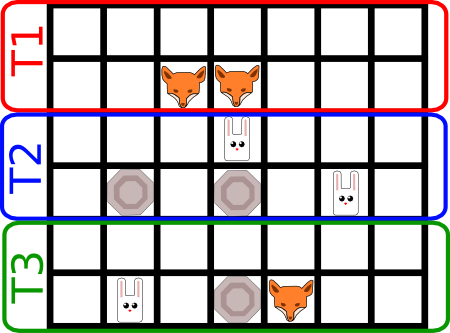
\includegraphics[height=1.6in]{grid1_par1.png}
    \end{subfigure}
    ~
    \begin{subfigure}[b]{0.4\textwidth}
      \centering
      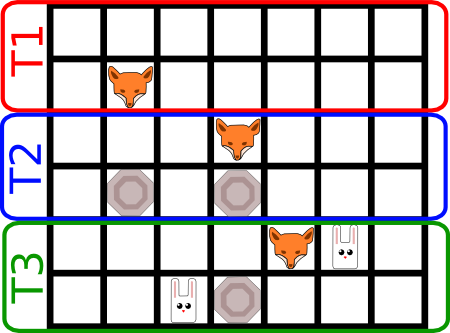
\includegraphics[height=1.6in]{grid2_par1.png}
    \end{subfigure}
    \caption{Divisão de trabalho da paralelização orientada à topologia}
    \label{fig:par1}
\end{figure}

A vantagem desta estratégia está na sua simplicidade. Além de não
necessitar de nenhum tipo de sincronização complexa, a comunicação
entre \textit{threads} é extremamente reduzida, cada \textit{thread}
só comunica com no máximo duas outras (a que contém a tira de cima e a
de baixo). Assim, os conflitos entre \textit{threads} são reduzidos (a
contenção de \textit{threads} é rara). Porém, esta estratégia tem
várias desvantagens. Primeiramente, como a divisão é estática, se o
\textit{input} não for balanceado podem surgir problemas de
escalabilidade (ainda que fosse possível aplicar as ideias que serão
usadas na estratégia mista para executar \textit{load
  balancing}). Além disso, devido ao facto que em cada iteração é
necessário percorrer a matriz da grelha por completo, a complexidade
temporal da simulação tem um \textit{bottleneck} no tamanho da grelha:
$R \times C$.

\subsection{Estratégia orientada aos dados}
Nesta estratégia o foco, como o próprio nome indica, é em paralelizar
os próprios dados. Por conseguinte, as unidades de trabalho
consideradas nesta estratégias são os próprios coelhos e
raposas. Inicialmente, os $N_1$ animais existentes são divididos de
uma forma \textit{round-robin} pelas \textit{threads} e guardados numa
estrutura de dados por cada \textit{threads} (uma \textit{queue}, por
exemplo). De modo a maximizar a localidade da distribuição, é feita
uma ordenação por posição (primeiro pela coordenada $y$ e depois pela
$x$, com o objetivo de ter uma distribuição semelhante à da estratégia
anterior) antes da divisão de trabalho. A distribuição está ilustrada
na Figura~\ref{fig:par2}, tendo como base o exemplo da secção
anterior. Após a divisão, a cada iteração a simulação é efetuada
considerando apenas os animais correspondentes a cada \textit{thread},
o que na prática corresponde a percorrer todos os elementos da
\textit{queue} de cada \textit{thread}. Apesar de só se considerarem
os animais existentes na geração atual, é mantida uma matriz que
representa a geração, com o objetivo de tornar mais eficiente certas
primitivas como o teste de quais células livres. Adicionalmente, é
necessário resolver os conflitos de movimentos. Para tal é mantida uma
segunda matriz que vai sendo preenchida com os animais nas novas
posições e que no fim servirá para cada \textit{thread} descartar os
animais que ou foram comidos ou que desapareceram num conflito. Nesta
matriz podem haver conflitos ao atualizar os seus valores e como tal é
necessário protegeras suas alterações usando
\textit{mutexes}. Experimentámos vários esquemas diferentes de
\textit{mutexes} para proteger a escrita nesta matriz, desde um
\textit{mutex} geral a um \textit{mutex} por célula, mas o que
funcionou melhor foi o de ter um \textit{mutex} por cada linha, o que
é justificável pelo facto da distribuição dos animais por
\textit{thread} ser feita pela ordem descrita anteriormente, o que faz
com que seja comum cada linha pertencer a apenas uma
\textit{thread}. Finalmente, assim como na estratégia anterior, as
\textit{threads} são sincronizadas usando barreiras depois da
simulação dos coelhos e depois da simulação das raposas.

\begin{figure}[H]
    \centering
    \begin{subfigure}[b]{0.4\textwidth}
      \centering
      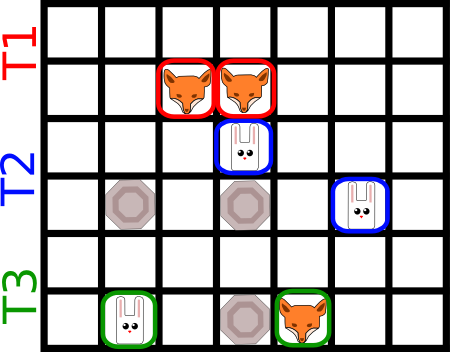
\includegraphics[height=1.6in]{grid1_par2.png}
    \end{subfigure}
    ~
    \begin{subfigure}[b]{0.4\textwidth}
      \centering
      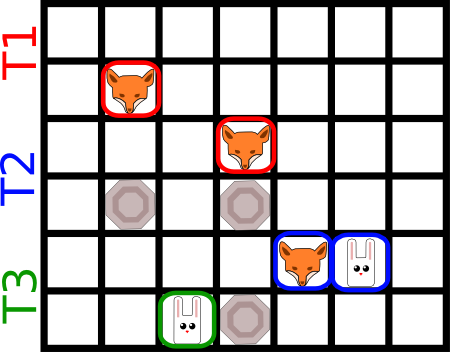
\includegraphics[height=1.6in]{grid2_par2.png}
    \end{subfigure}
    \caption{Divisão de trabalho da paralelização orientada aos dados}
    \label{fig:par2}
\end{figure}

Esta estratégia destaca-se da anterior por apenas fazer os cálculos
estritamente necessários por iteração. Assim, o \textit{bottleneck}
temporal de simular a geração $i$ é da ordem de $N_i$. Porém, para se
conseguir esta melhoria, o algoritmo base ficou mais complexo através
da presença das várias \textit{queues} e da forma de sincronização das
\textit{threads}. Ao contrário da estratégia orientada à topologia,
rebalancear o trabalho é muito mais natural para esta estratégia,
basta movimentar unidades de trabalho entre as \textit{queues} de cada
\textit{thread}. Discutiremos com mais detalhes alternativas possíveis
para o processo de \textit{load balancing} no fim desta secção.

\subsection{Estratégia mista}
A última estratégia que explorámos considera o melhor das duas
estratégias anteriores. Por um lado a divisão efetuada é análoga à da
estratégia orientada à topologia, onde se definem tiras horizontais
para serem atribuídas a cada \textit{thread}. Por outro lado, são
mantidas \textit{queues} por cada \textit{thread} como na estratégia
orientada aos dados de modo a apenas percorrer os elementos relevantes
para a simulação da iteração atual. Adicionalmente, as tiras
atribuídas a cada \textit{thread} não são uniformes como na estratégia
original, mas tentam equilibrar o número de animais associadas a cada
\textit{thread}. Assim, é feita uma divisão usando um algoritmo
\textit{greedy} que vai crescendo cada tira até que ela inclua pelo
menos $\frac{N_1}{T}$ animais, sendo $T$ o número de
\textit{threads}. Esta distribuição está ilustrada
na Figura~\ref{fig:par3}, tendo como base o exemplo da secção
anterior.

\begin{figure}[H]
    \centering
    \begin{subfigure}[b]{0.4\textwidth}
      \centering
      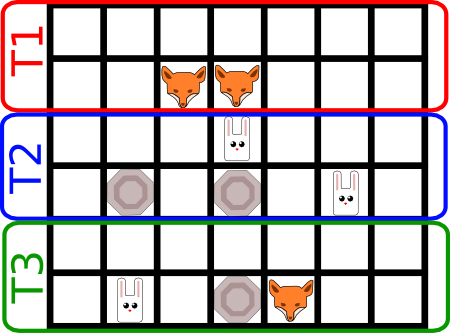
\includegraphics[height=1.6in]{grid1_par3.png}
    \end{subfigure}
    ~
    \begin{subfigure}[b]{0.4\textwidth}
      \centering
      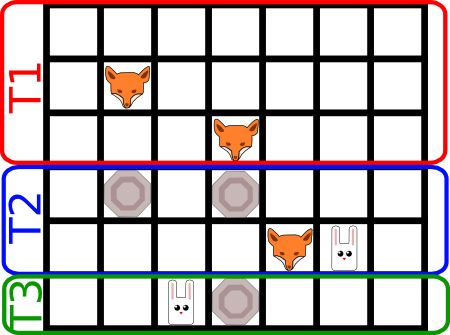
\includegraphics[height=1.6in]{grid2_par3.png}
    \end{subfigure}
    \caption{Divisão de trabalho da paralelização mista}
    \label{fig:par3}
\end{figure}

Esta estratégia mantêm a vantagem de comunicações reduzidas entre
\textit{threads} que a primeira estratégia possuía, ao mesmo tempo que
mantém o \textit{bottleneck} temporal a $N_i$ para a geração $i$. Com
esta nova divisão também se torna mais fácil rebalancear o trabalho,
basta delinear novas tiras respeitando as condições já referidas (de
ter aproximadamente $\frac{N_1}{T}$ animais por tira) e atualizar as
\textit{queues} respetivas.

\subsection{Rebalanceamento de trabalho}
Para as estratégias que permitem uma divisão dinâmica de trabalho
começamos por descrever um conjunto de observações
importantes. Primeiro, é importante notar que quando é feita uma
redistribuição de trabalho, não é viável que esta não seja global, ou
seja, que não inclua todas as \textit{threads}. Isto é devido ao facto
que é importante sincronizar o trabalho de cada uma após cada parte da
simulação, logo mesmo que alguma \textit{thread} não participasse na
redistribuição de trabalho teria de ficar à espera que as restantes
terminassem. Isto elimina vários tipos de estratégias clássicas como
\textit{work sharing} entre \textit{threads}. Outra observação
importante passa por notar que não é eficiente redistribuir o trabalho
a cada iteração, pois ambas as estratégias dinâmicas usam algoritmos
pesados temporalmente para redistribuição de trabalho. Além disso,
obter o valor de $N_i$ para decidir o quão desbalanceadas estão as
\textit{queues} também requer um algoritmo pesado, logo também é pouco
eficiente fazê-lo a cada iteração. Assim, optámos por apenas
redistribuir trabalho a cada $\sqrt{N_G}$ gerações, no máximo. Antes
de efetuar a redistribuição, aglomera-se o valor de $N_i$ somando o
tamanho de todas as \textit{queues} e se alguma das \textit{queues}
tiver mais de $25\%$ elementos do que $\frac{N_i}{T}$ então é feita
uma redistribuição. O valor de $25\%$ foi obtido empiricamente.

%----------------------------------------------------------------------------------------
%	SECTION 4
%----------------------------------------------------------------------------------------

\section{Resultados e discussão}
\label{sec:res}


%----------------------------------------------------------------------------------------
%	SECTION 5
%----------------------------------------------------------------------------------------

\section{Conclusão e notas finais}
\label{sec:con}

%\bibliographystyle{plain}
%\bibliography{report}

\end{document}
